\chapter{Audit de clefs cryptographiques}

\section{Introduction}
Cette première partie du projet consiste à faire une étude des clefs cryptographiques RSA circulant sur Internet. Nous avons donc dans un premier temps récupéré une liste d'adresses IP dont le port 443 (HTTPS) était ouvert.\\


Ensuite, nous avons tenté de récupérer les certificats de toutes les adresses listées. Cette récupération s'occupait également d'extraire les moduli et les clefs publiques des certificats, mais aussi de stocker une liste de certificats doublons.\\


Enfin, avec tous les moduli que nous avons extraits, nous avons pu construire deux arbres permettant de définir si des moduli contiennent des facteurs premiers communs.

\section{ZMAP}

ZMAP est un outil permettant de faire des scans réseau.  Il est capable de scanner toutes les adresses IPv4 possibles, avec une moyenne de 1.4 millions de paquets envoyés par secondes sur les connexions à très haut débit. Nous l'avons utilisé pour scanner l'ensemble des adresses IPv4, en envoyant simplement des paquets SYN aux adresses visées sur le port 443 pour SSL.\\


Pour l'installer sur nos machines, voici la procédure à suivre :
\begin{enumerate}
\item Installation des dépendances :
\begin{verbatim}
~ $ sudo apt-get install cmake libgmp3-dev libpcap-dev gengetopt byacc flex git
\end{verbatim}
\item Récupération des sources de ZMap :
\begin{verbatim}
~ $ git clone git://github.com/zmap/zmap.git
\end{verbatim}
\item Compilation :
\begin{verbatim}
~ $ cd zmap
~/zmap $ mkdir build
~/zmap $ cd build
~/zmap/build $ cmake .. -DENABLE_HARDENING=ON
~/zmap/build $ make
~/zmap/build $sudo make install
\end{verbatim}
\end{enumerate}

Il y a plusieurs options disponibles, nous avons utilisé la commande suivante pour effectuer notre scan :
\begin{verbatim}
# zmap -p 443 -o scan_output_zmap
\end{verbatim}

\section{Application RC}

Une fois que l'on avait la liste d'adresses fournie par ZMAP, il nous restait à récupérer les certificats sur les serveurs dont le port HTTPS était ouvert, en établissant une connexion sur chacun d'eux.\\

\subsection{Récupération des certification}

Nous avons codé un scripts perl pour la récupération de certificats SSL (ssl\_collector.pl), suivant l'algorithme \ref{alg:recupCertif}.\\


\begin{algorithm}[H]
\label{alg:recupCertif}
 %\SetAlgoLined % For previous releases [?]
 \Entree{Fichier f, contenant les adresse ayant le port 443 ouvert}
 \Sortie{Certificats et clé de session des adresses}
 \Donnees{log, certificat, clé de session}
 
 \PourTous{adresses de f}{
	Se connecter au serveur\;
	\eSi{echec}{
		\Si{le log contient \textit{protocol}}{
	 		on incrémente le nombre d'échecs de protocoles\;
	 	}
	 	\Si{le log contient \textit{handshake}}{
	 		on incrémente le nombre d'échecs de poignée de main\;
		}
	}{
	On capture la session (dont le certificat serveur)\;
	\Si{!echec de capture de session}{
		on extrait le certificat et la clé de session\;
	}	 
	}
}

\Retour{certificats et clés de session}
\caption{Récupération des certificats} 
\end{algorithm}
\vspace{0.7cm}


Commandes OpenSSL utilisées :
\begin{itemize}
\item pour l'établissement de la connexion (avec s\_client) :
\begin{verbatim}
$ echo  \" \" | timeout 20 openssl s_client -connect $addr:443 -sess_out tmp_$addr.pem 
-ignore_critical -showcerts -CApath /etc/ssl/certs > /dev/null 2> tmp_$addr.log
\end{verbatim}

\item  pour la capture de session (avec sess\_id) :
\begin{verbatim}
$ openssl sess_id -in tmp_$addr.pem -cert > certs/$addr.pem 2> tmp_$addr.log
\end{verbatim}

\item pour la récupération du certificat et de la clé privée :
\begin{verbatim}
$ openssl x509 -in certs/$addr.pem -noout -pubkey > keys/$addr.pem 2> tmp_$addr.log
\end{verbatim}
\end{itemize}


\subsection{Gestion des doublons}

Pour ce qui est de la gestion des doublons, nous avons également créé un autre script perl (\texttt{clean.pl}). Le concept est simple, nous allons stocker l'ensemble des empreintes des certificats dans un dossier spécifique (certs\_doublons). Si une empreinte se trouve déjà dans le dossier, on la stocke dans un autre dossier contenant les doublons (à l'aide de comparaisons sur les liens symboliques).\\


\begin{algorithm}[H]
\label{alg:clean}
 %\SetAlgoLined % For previous releases [?]
 \Entree{Pré-requis : Exécution de l'algorithme ssl\_collector \\
 Création d'un dossier D contenant les certificats à traiter}
 \Sortie{Dossiers : certs\_doublons, certs\_links; Fichier : moduli}
 \Donnees{Certificats C; Fingerprint F; Chaîne de caractères S; Modulo M}
 certs\_doublons $\leftarrow$ dossier\_vide\;
 certs\_links $\leftarrow$ dossier\_vide\;
 moduli $\leftarrow$ fichier\_vide\;
 \PourTous{C $\in$ D}{
 	F $\leftarrow$ \textit{fingerprint}(C)\;
 	S $\leftarrow$ \textit{nom\_fichier}(C)\;
 	M $\leftarrow$ \textit{modulo}(C)\;
 	\Si{échec(F)}{
 		continue\;
 	}
 	\eSi{F $\in$ certs\_links}{
 		certs\_doublons/F $\leftarrow$ concat(certs\_doublons/F, S)\;
 	}{
 		moduli $\leftarrow$ concat(moduli, M)\;
 		certs\_links $\leftarrow$ F\;
 	}
 }
 \caption{Gestion des doublons} 
\end{algorithm}
\vspace{0.7cm}

Commandes OpenSSL utilisées :
\begin{itemize}
\item pour la récupération du \textit{fingerprint} :
\begin{verbatim} 
$ openssl x509 -noout -in $file -modulus 2> /dev/null | cut -d'=' -f2 |
 sha512sum | cut -d' ' -f1 2> /dev/null 
\end{verbatim}

\item pour savoir le \textit{fingerprint} se trouve dans \textit{certs\_links} :
\begin{verbatim} 
$ ls -l certs_links | grep $hash 2> /dev/null
\end{verbatim}

\item pour ajouter le modulo dans le fichier \textit{moduli} :
\begin{verbatim} 
$ openssl x509 -noout -in $file -modulus 2> /dev/null | cut -d'=' -f2 >> moduli 
\end{verbatim}

\item Pour créer un lien symbolique dans \textit{certs\_links}
\begin{verbatim} 
$ ln -s ../$file certs_links/$hash > /dev/null 2> /dev/null
\end{verbatim}
\end{itemize}


\section{Factorisation}



\subsection{Algorithmes}

L'objectif final de cette première partie était de déterminer s'il existait des facteurs premiers communs parmi les clefs récupérées. Pour cela nous avons développé deux arbres de factorisation.
Lors du scan nous avons récupéré 85 000 certificats uniques, mais nous avons également souhaité faire la factorisation avec les données du projet Sonar de Rapid7 Labs avec 523 000 certificats.\\


Le premier arbre se contente de multiplier l'ensemble des moduli par groupe de deux.
Le second arbre calcule deux modulos du résultat produit, selon le carré des résulats stockés par l'arbre des produits (aux étapes intermédiaires).\\


Une fois le second arbre calculé, les dernières feuilles des arbres indiquent soit un $PGCD(\text{res\_final}, N_i ) = 1$ (donc avec des entiers premiers uniques), ou un $PGCD(\text{res\_final}, N_i ) = p$ (entier premier non unique).\\


Voici les algorithmes de ces deux arbres :\\


\begin{algorithm}[H]
\label{alg:productTree}
 %\SetAlgoLined % For previous releases [?]
 \Entree{Tableau des moduli des clefs publiques : T}
 \Sortie{Hauteur de l'arbre, produits des moduli des clefs publiques}
 \Donnees{Tableaux v, tmp; Entier i, level}
 $v \leftarrow T$\;
 $level \leftarrow 0$\;
 \Tq{$|v|>1$}{
  $tmp \leftarrow \emptyset$\;
  \PourCh{$i \in \{0, .., |v| / 2\}$}{
    $tmp[i] \leftarrow v[i\times2] \times v[i\times2 + 1]$\;
  }
  $storeProductLevel(v, level)$\;
  $v \leftarrow tmp$\;
  $level \leftarrow level + 1$\;
 }
 \Retour{level}
 \caption{Construction de l'arbre des produits} 
\end{algorithm}
\vspace{0.7cm}



\begin{algorithm}[H]
 \label{alg:remainderTree}
 %\SetAlgoLined % For previous releases [?]
 \Entree{Hauteur de l'arbre des produits : level}
 \Sortie{PGCDs des moduli des clefs publiques}
 \Donnees{Tableaux P, v, w; Entier i}
 $P \leftarrow getProductLevel(level)$\;
 \Tq{$level>0$}{
  $level \leftarrow level - 1$\; 
  $v \leftarrow getProductLevel(level)$\;
  \PourCh{$i \in \{0, .., |v|\}$}{
    $v[i] \leftarrow P[i/2] \pmod{v[i]^2}$\;
  }
  $storeRemainderLevel(v, level+1)$\;
  $v \leftarrow tmp$\;
 }
 $w \leftarrow \emptyset$\;
 \PourCh{$i \in \{0, .., |v|\}$}{
    $w[i] \leftarrow P[i/2] \pmod{v[i]^2}$\;
    $w[i] \leftarrow w[i] / v[i]$\;
    $w[i] \leftarrow pgcd(w[i],v[i])$\;
  }
 \Retour{w}
 \caption{Construction de l'arbre des restes}
\end{algorithm}
\vspace{0.7cm}


\subsection{Implémentation}


Lors de nos tâches d'optimisation, nous avons réalisé qu'il était possible de construire l'arbre entier (\textit{product tree} + \textit{remainder tree}), en mémoire vive (nous avons donc créé une option fullRAM à notre algo).\\


L'algorithme est le même, seul le choix de la structure change.
Dans la première méthode, nous utilisions des fichiers binaires GMP à chaque étape de construction, dans la  seconde nous stockons l'intégralité de l'arbre des produits en mémoire.\\


Pour accélérer la construction de l'arbre, nous utilisons des \textit{threads}, qui parallélisent le traitement de chaque niveau d'arbre (sur la largeur de l'arbre).
Nous avons tenté d'améliorer encore le procédé, en parallélisant le calcul sur la hauteur de l'arbre. Il s'est avéré que ce n'était pas aussi efficace à cause des dépendances entre les niveaux, nous avons donc abandonné cette partie.\\


Nous allons dans cette partie expliciter les composantes principales implémentées en mémoire de l'algorithme de factorisation.  Nous développerons notamment la méthode \texttt{computeSuperSpeed}, qui prend en entrée un nom de fichier, contenant la liste des moduli. 


\subsubsection{Initialisation}

\begin{lstlisting}[style=customc,caption=fact\_superspeed.c - partie 1, label=fact1]
	vec_t v = {0};
	transformFile(input);
	char *moduli_filename = "PInterm1";
	input_bin_array(&v, moduli_filename);
	
	int count = v.count;
	int levels_count = (int) ceil (log (count) / log (2)) + 1;
	product_tree.levels_count = levels_count;
	
	product_tree.levels = (vec_t *) malloc (levels_count * sizeof (vec_t));
	product_tree.levels[0] = v;
	int count_i = count / 2;
	for (int i = 1; i < levels_count; i++) {
		init_vec (product_tree.levels + i, count_i);
		product_tree.levels[i].count = count_i;
		count_i = count_i / 2;
	}
	printf ("Done.\n\n");
\end{lstlisting}

Dans cette fraction de méthode, on initialise les différentes variables :
\begin{itemize}
	\item le fichier contenant les moduli au format binaire est chargé, dans le vecteur \texttt{v}. Le vecteur est une structure décrit par son nombre d'éléments et par une liste de \texttt{mpz\_t} ;
	\item on calcule le nombre de niveaux à dérouler charger, considérant que l'arbre est binaire ;
	\item on initialise enfin les vecteurs de la structure \texttt{product\_tree}. Il s'agit d'une structure représentant  l'arbre des produit, composée d'une hauteur d'arbre et d'une liste de vecteurs.
\end{itemize}



\subsubsection{Calcul de l'arbre des produits}

\begin{lstlisting}[style=customc,caption=fact\_superspeed.c - partie 2, label=fact2]
	for (int i = 1; i < levels_count; i++) {
		vec_t *w = product_tree.levels + i;
		vec_t *v2 = product_tree.levels + i - 1;
		void mul_job(int i) {
			mpz_mul(w->el[i], v2->el[2*i], v2->el[2*i+1]);
		}
		iter_threads(0, v2->count/2, mul_job);

		if (v2->count & 1)
			mpz_set(w->el[v2->count/2], v.el[v2->count-1]); 

	}
\end{lstlisting}

Le déroulement de l'arbre des produits est plutôt simple. Les éléments connexes sont multipliés à chaque niveau puis le résultat est stocké dans le niveau suivant correspondant. On remarque également la méthode de parallélisation sur cette boucle afin d'accélérer la multiplication.\\

Nous avons pensé à intégrer des améliorations pour couper des branches inutiles, ou encore accélérer le développement de l'arbre en parallélisant également en hauteur, mais ces opérations se sont avérées inutiles car elles nécessitaient la mise en place de tests qui ralentissaient l'exécution du programme. L'opération de multiplication n'est en effet que très légèrement gourmande en processus, nous avons décidé de garder un développement d'arbre le plus épuré possible.\\




\subsubsection{Calcul de l'arbre des restes}

\begin{lstlisting}[style=customc,caption=fact\_superspeed.c - partie 3, label=fact3]
	int secL;
	int sizeP=1; 
	vec_t *modPre = product_tree.levels + product_tree.levels_count - 1;
	vec_t modCur,*prodL,gcd;
	secL = product_tree.levels_count;
	
	do {
		sizeP *= 2; 
		init_vec(&modCur,sizeP);	
	

		prodL = product_tree.levels + secL - 2;
		void mul_job(int j){			
			mpz_pow_ui(prodL->el[j],prodL->el[j],2); 
			mpz_mod(modCur.el[j],modPre->el[j/2],prodL->el[j]); 	
		}
		iter_threads(0, prodL->count, mul_job);
		
		*modPre = modCur;
		free_vec (prodL);	
	} while (--secL > 1);

\end{lstlisting}

Le calcul de l'arbre des restes se fait aussi efficacement. On récupère de l'arbre des restes le produit correspondant au niveau équivalent de celui de l'arbre des restes, produit que l'on élève au carré. On effectue ensuite le calcul modulaire requis suivant l'algorithme. On remarque également le \textit{multi-threading} effectué. Durant ce calcul, on ne conserve en mémoire que le niveau $j$ et $j-1$ de l'arbre des restes, afin de ne pas surcharger la mémoire. \\



\subsubsection{Dernière étape de l'arbre des restes}

\begin{lstlisting}[style=customc,caption=fact\_superspeed.c - partie 4, label=fact4]
init_vec(&gcd,modCur.count);
	
	input_bin_array (&v, moduli_filename);
	void mul_job(int j){
		mpz_divexact(modCur.el[j],modCur.el[j],v.el[j]); 
		mpz_gcd (gcd.el[j],modCur.el[j],v.el[j]); 
	}
	iter_threads(0, v.count, mul_job);
\end{lstlisting}

Afin de ne pas avoir à ajouter des tests dans la boucle principale, nous avons séparé la dernière étape du calcul de l'arbre des restes. En effet, cette étape s'accompagne d'une division et d'un calcul de PGCD qui peuvent eux aussi être parallélisés. \\





\subsubsection{Identification des moduli vulnérables}
Il convient enfin d'analyser les PGCD obtenus. Dans un premier temps, on récupère tous les PGCD étant différents de 1, que l'on stocke dans un vecteur de moduli potentiellement vulnérables. De plus, si celui-ci est premier, alors on stocke ce premier dans un vecteur spécifique : \verb+potentielVuln+. 

\begin{lstlisting}[style=customc,caption=fact\_superspeed.c - partie 5a, label=fact5]
	vec_t potentielVuln, premiers;
	init_vec (&potentielVuln, gcd.count);
	init_vec (&premiers, gcd.count);
	mpz_t q;
	mpz_init (q);
	
	int pvuln = 0, ppremier = 0;
	for (int i = 0; i < gcd.count; i++) {
		if (mpz_cmp_ui (gcd.el[i], 1) != 0) {
			mpz_set (potentielVuln.el[pvuln++], v.el[i]);
			if (mpz_probab_prime_p (gcd.el[i], 25) != 0) {
				mpz_set (premiers.el[ppremier++], gcd.el[i]);
			}
		}
	}
\end{lstlisting}


Enfin, on récupère tous les moduli vulnérables potentiels étant divisibles par un premier récupéré. On en profite également pour récupérer $q$ où $\text{moduli}=p*q$ avec $p$ étant le premier récupéré. On écrit ces éléments dans un fichier : \verb+moduli_p_q+. 
\begin{lstlisting}[style=customc,caption=fact\_superspeed.c - partie 5b, label=fact5]
    	potentielVuln.count = pvuln;
	premiers.count = ppremier;

	FILE *result = fopen ("moduli_p_q", "w");
	start = now ();
	for (int i = 0; i < potentielVuln.count; i++) {
		for (int j = 0; j < premiers.count; j++) {
			if (mpz_divisible_p (potentielVuln.el[i], premiers.el[j]) != 0) {
				mpz_divexact (q, potentielVuln.el[i], premiers.el[j]);
				if (mpz_probab_prime_p (q, 25) != 0) {
					if (input_type == INPUT_HEXA) 
						gmp_fprintf (result, "%ZX, %ZX, %ZX\n", potentielVuln.el[i], premiers.el[j], q);
					else
						gmp_fprintf (result, "%Zd, %Zd, %Zd\n", potentielVuln.el[i], premiers.el[j], q);
				}
			}
		}
	}

\end{lstlisting}






\subsubsection{Compilation}
Pour compiler le programme :
\begin{verbatim}
~ $ sudo apt-get install libgmp-dev cmake git 
~ $ git clone https://github.com/RandomGuys/fact.git
~ $ cd fact
~/fact $ mkdir build
~/fact $ cd build
~/fact/build $ cmake ..
~/fact/build $ make
~/fact/build $ sudo make install
\end{verbatim}

Il y a également un \textit{man} qui s'installe, vous pouvez donc consutler l'aide avec la commande \verb+man fact+.

Pour utiliser ce programme, la ligne de commande est la suivante :
\begin{verbatim}
$ fact -m mes_moduli --fullram|--files [--format hexa|decimal]
\end{verbatim}


\section{Conclusion des résultats produits}

\subsection{Fichier de résultats}
Les résultats se trouvent dans le fichier \verb+moduli_p_q+ construit de la façon suivante :
\begin{verbatim}
modulus, facteur commun, facteur déduit
...
\end{verbatim}
\subsection{Premiers chiffres}
Voici les premiers chiffres obtenus des scans :


\begin{table}[H]
\centering
\begin{tabular}{|r|c|c|}
\hline
\textbf{}&\textbf{Scan 1}&\textbf{Scan Sonar}\\
\hline
\textbf{moduli}&85 636&523 017\\
\hline
\textbf{vulnérables}&104 (0,12\%)&2 382 (0,46\%)\\
\hline
\textbf{facteurs communs}&11&757\\
\hline
\textbf{autres facteurs}&104&2 382\\
\hline
\textbf{total facteurs}&115&3 139\\
\hline
\end{tabular}

\caption{Résultats globaux obtenus}
\label{res}
\end{table}

En comparant avec les résultats du projet \textit{factorable} de l'Université de Californie et de l'Université du Michigan, nous obtenons un pourcentage de clefs vulnérables assez proche. En effet, ils ont obtenu 0,50\% de clefs vulnérables et nous en avons trouvées 0,46\% \\


Pour la suite de l'analyse des résultats, nous nous sommes focalisés sur le scan Sonar.

\subsection{Entropie}
Le graphe suivant représente le pourcentage d'entropie des 757 facteurs premiers trouvés. Ce niveau d'entropie a été calculé selon l'entropie de Shannon (représentation binaire des clefs). Nous nous sommes basés sur la bibliothèque \verb+libdisorder+ (\url{http://libdisorder.freshdefense.net/}) qui fournit un programme de tests. Ce dernier a été modifié pour nos besoins et pour pouvoir injecter les résultats dans gnuplot pour obtenir le graphe suivant :

\begin{figure}[H]
\centering
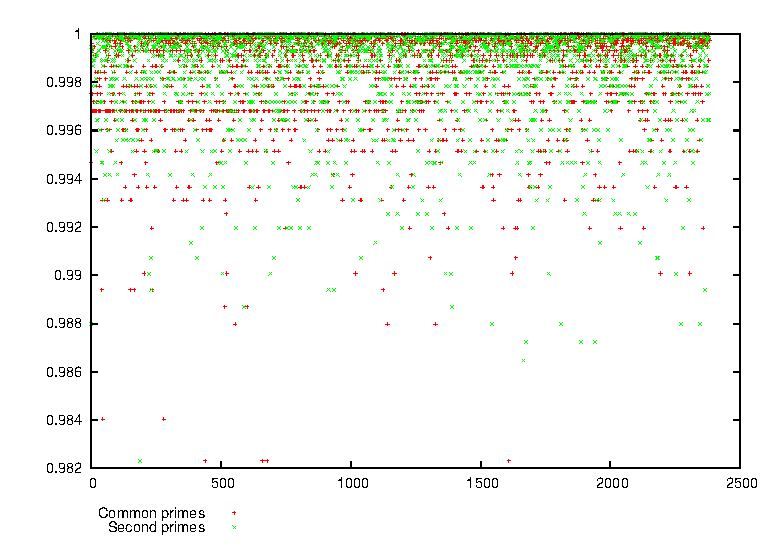
\includegraphics[width=16cm]{images/entropyprimes.eps}
\caption[Entropie moyenne]{Entropie moyenne des facteurs communs : 0.998518 - Entropie moyenne des second facteurs : 0.998551}
\label{entropiePrime}
\end{figure}


\subsection{Tailles des clefs}
Dans nos résultats, nous pouvons constater que seules deux tailles de clefs apparaissent : 512 et 1024 bits. Voici les chiffres :


\begin{table}[H]
\centering
\begin{tabular}{|r|c|c|}
\hline
\textbf{}&\textbf{512 bits}&\textbf{1024 bits}\\
\hline
\textbf{Total}&2 345&318 558\\
\hline
\textbf{Vulnérables}&6 (0,26\%)&2 376 (0,75\%)\\
\hline
\end{tabular}
\caption{Tailles de clés obtenues}
\label{tailles}
\end{table}


Nous avions également d'autres tailles de clefs en entrée mais leur nombre devait être trop petit par rapport à l'espace des clefs de cette taille pour obtenir des facteurs communs.


